\chapter{Analysis evaluation} \label{chr:analysisEvaluation}

This chapter consists of five example analyses - three for the W-L test and two for the LA analysis. In each case, the inputs and results of the test are defined, and the entire process is concluded with the author's commentary on the analysis. 

\section{WL test}

\subsection{Pylinac Demo}

Pylinac has a built-in demo which can be started by calling the appropriate function. Sample images are then loaded and the W-L test is performed in the standard way.

\subsubsection{Inputs}

\begin{itemize}
    \item 17 test images
    \item BB size of 5 mm
\end{itemize}

\subsubsection{Numerical results}

\begin{multicols}{2}
\begin{itemize}

    \item Couch shift instructions: LEFT 0.05mm; OUT 0.26mm; DOWN 0.20mm
    \item Maximum 2D CAX to BB distance: 1.24mm
    \item Median 2D CAX to BB distance: 0.69mm
    \item Mean 2D CAX to BB distance: 0.62mm
    \item Maximum 2D CAX to EPID distance: 2.36mm
    \item Median 2D CAX to EPID distance: 1.31mm
    \item Mean 2D CAX to EPID distance: 1.26mm
    \item Gantry 3D isocenter diameter: 1.03mm
    \item Maximum Gantry RMS deviation: 1.01mm
    \item Maximum Collimator RMS deviation: 0.78mm
    \item Maximum Couch RMS deviation: 1.24mm
    \item Maximum EPID RMS deviation: 1.32mm
    \item Gantry + Collimator 3D isocenter diameter: 1.10mm
    \item Collimator 2D isocenter diameter: 1.08mm
    \item Couch 2D isocenter diameter: 2.35mm
    
\end{itemize}
\end{multicols}

\subsubsection{Plots}

\begin{figure}[H]
    \centering
    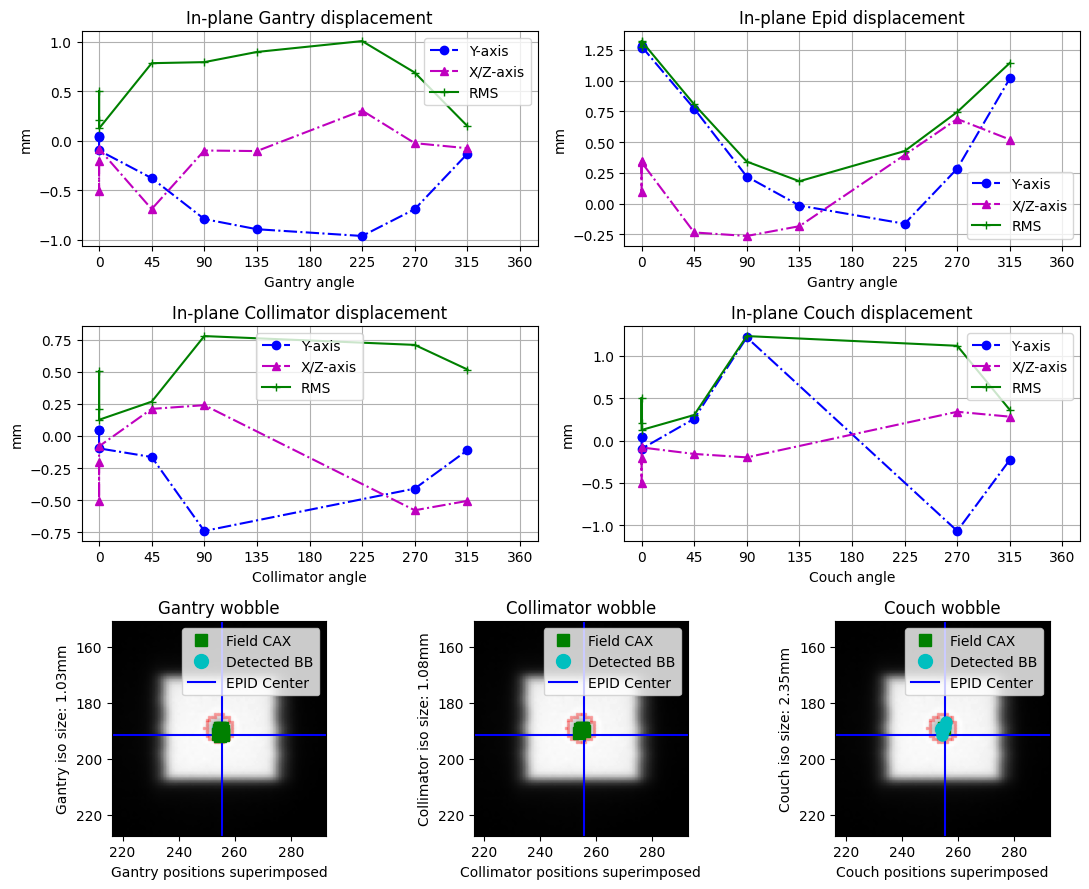
\includegraphics[width=0.85\textwidth]{Content/Images/analysis_wl_demo_summary_plot.png}
    \caption{Summary plot of demo test}
\end{figure}

\begin{figure}[H]
    \centering
    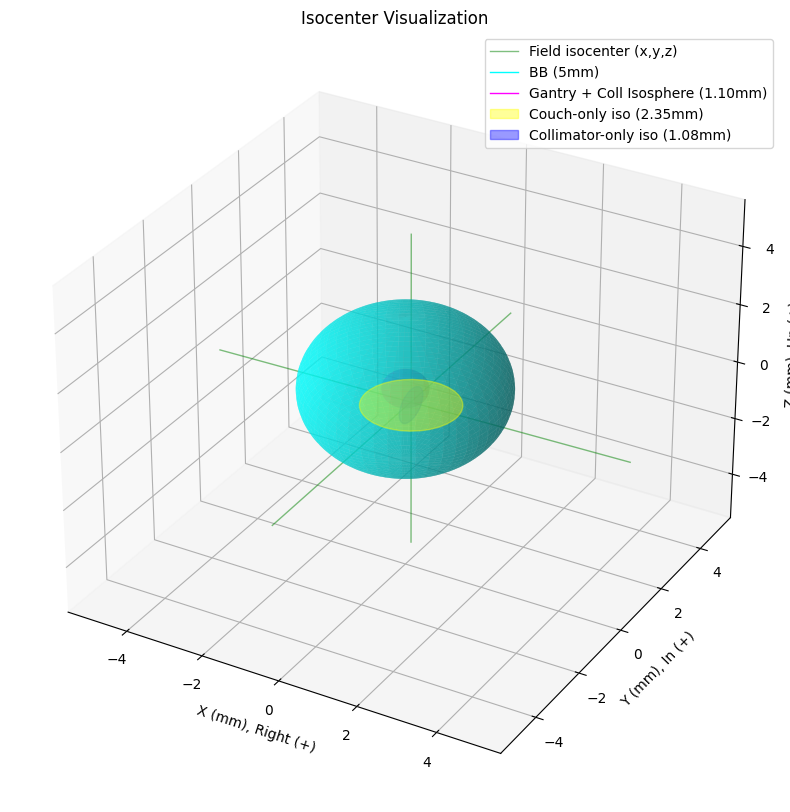
\includegraphics[width=0.6\textwidth]{Content/Images/analysis_wl_demo_isocenter_plot.png}
    \caption{Isocenter plot of demo test}
\end{figure}

\subsubsection{Analysis}

As can be seen, the results obtained indicate that the module is working correctly. The results are consistent with those published in the module's documentation \cite{pylinac_wl_demo}. 

\subsection{Test on real images} \label{sec:analysisEvaluationWLRealImagesOncology}

This analysis is conducted on real DICOM images obtained from a W-L test session at the National Institute of Oncology in Kraków (\autoref{sec:envSetupOncologyKrakow}).

\subsubsection{Inputs}

\begin{itemize}
    \item 22 images with dimensions 640x640 px.
    \item BB size of 2mm
\end{itemize}

\begin{figure}[H]
    \centering
    \fbox{
\includegraphics[width=0.4\textwidth]{Content/Images/analysis_wl_oncology_example_input.png}}
    \caption{One of the input images}
\end{figure}

\subsubsection{Numerical results}

\begin{multicols}{2}
\begin{itemize}

    \item Couch shift instructions: LEFT 0.06mm; IN 0.23mm; DOWN 0.09mm
    \item Maximum 2D CAX to BB distance: 0.99mm
    \item Median 2D CAX to BB distance: 0.34mm
    \item Mean 2D CAX to BB distance: 0.51mm
    \item Maximum 2D CAX to EPID distance: 1.07mm
    \item Median 2D CAX to EPID distance: 0.44mm
    \item Mean 2D CAX to EPID distance: 0.58mm
    \item Gantry 3D isocenter diameter: 0.26mm
    \item Maximum Gantry RMS deviation: 0.29mm
    \item Maximum Collimator RMS deviation: 0.34mm
    \item Maximum Couch RMS deviation: 0.99mm
    \item Maximum EPID RMS deviation: 0.43mm
    \item Gantry + Collimator 3D isocenter diameter: 0.48mm
    \item Collimator 2D isocenter diameter: 0.33mm
    \item Couch 2D isocenter diameter: 1.33mm
    
\end{itemize}
\end{multicols}

\subsubsection{Plots}

\begin{figure}[H]
    \centering
    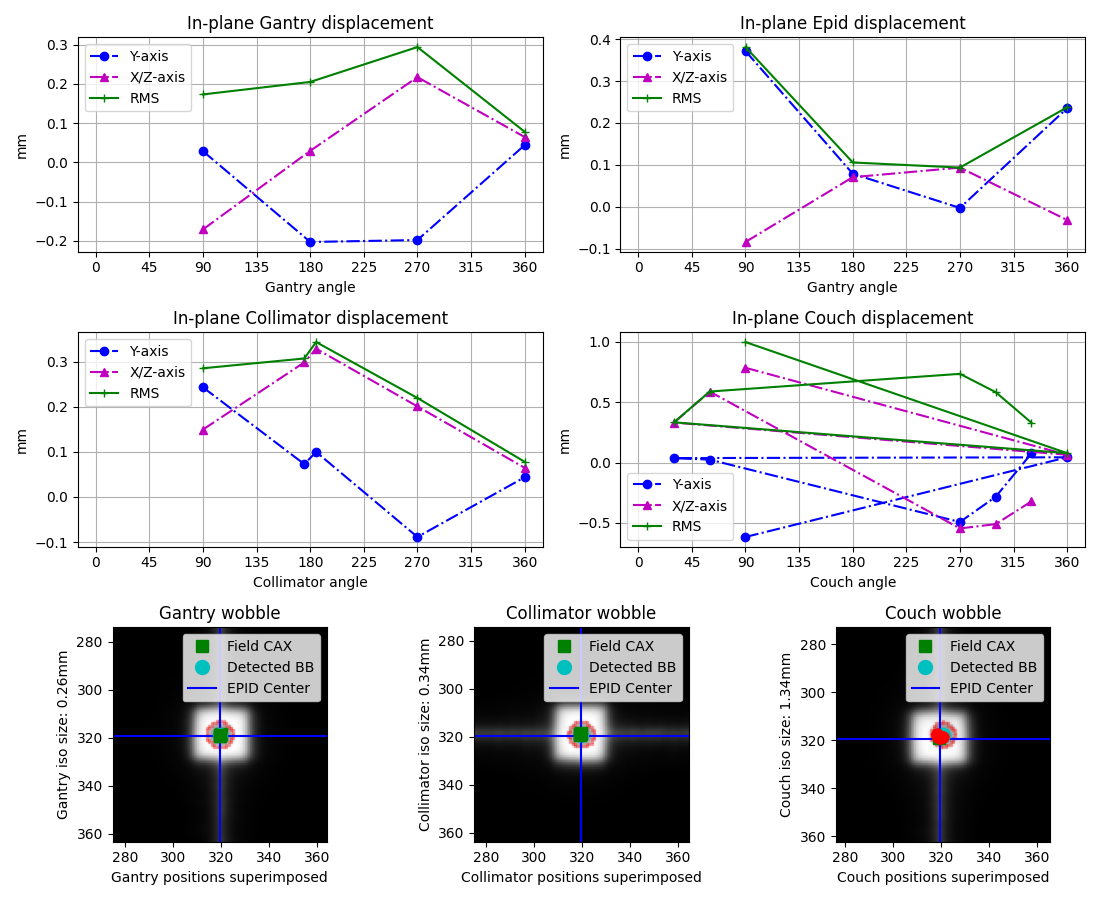
\includegraphics[width=0.85\textwidth]{Content/Images/analysis_wl_oncology_summary_plot.png}
    \caption{Summary plot of test on real images}
\end{figure}

\begin{figure}[H]
    \centering
    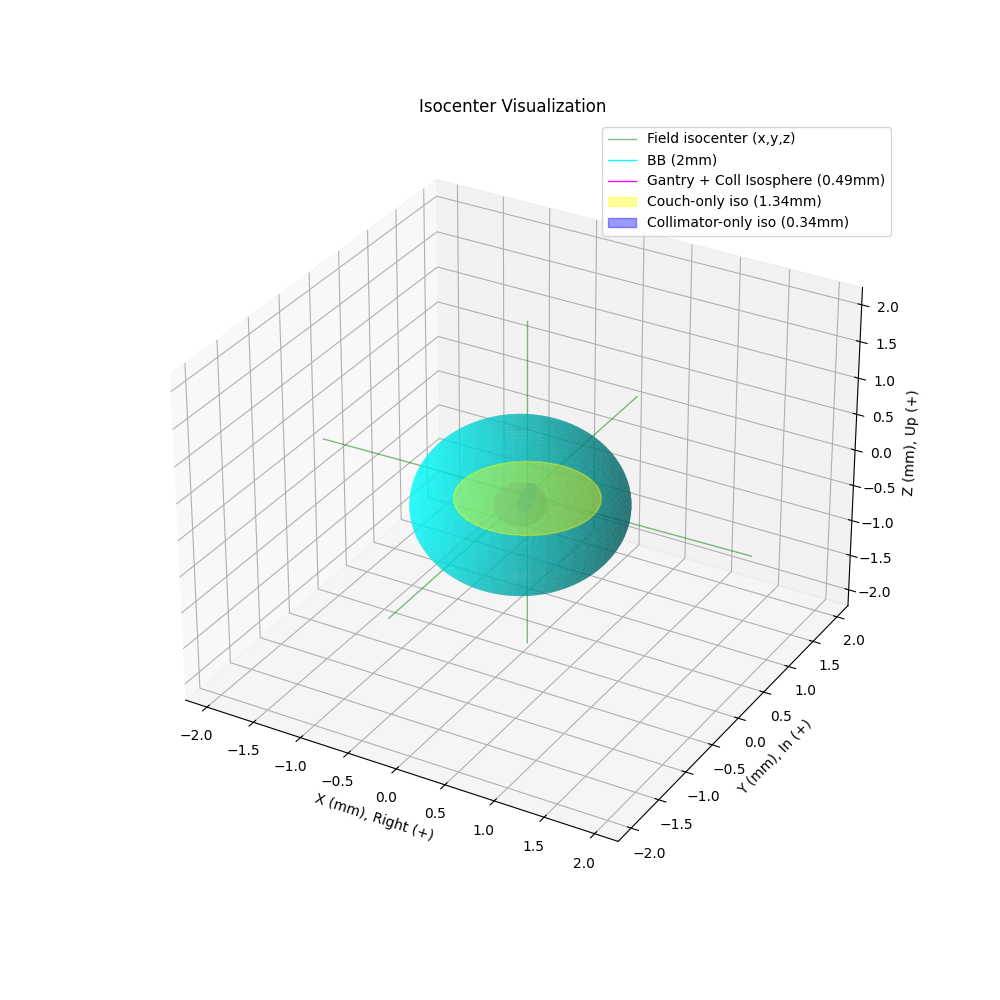
\includegraphics[width=0.60\textwidth]{Content/Images/analysis_wl_oncology_isocenter_plot.png}
    \caption{Isocenter plot of test on real images}
\end{figure}

\subsubsection{Analysis}

As can be observed, the displacement values are relatively small, both in terms of the shift instructions and the individual detected BB distances from the CAX from which they result. This aligns with the initial hypothesis, as an examination of the images manually reveals that the BB is situated close to the centre of the radiation field in all images. Additionally, the visualisation of isocenters demonstrates that they are properly aligned. Consequently, it can be concluded that the machine has been correctly calibrated.

\subsection{Test on artificial images}

This analysis is conducted on a generated set of images that have been modified using Pylinac's Offset BB function, which was originally developed for use in benchmarking. \cite{pylinac_benchmarking}. This method involves artificially moving the detected BB by a given distance in space, to evaluate the impact of this manipulation on the results.

\subsubsection{Inputs}

\begin{itemize}
    \item 18 generated images, where the position of BB has been shifted 2 mm in Y direction, 4 mm in X direction, and 6 mm in Z direction
    \item BB size of 4 mm
\end{itemize}

\subsubsection{Numerical results}

\begin{itemize}

    \item Couch shift instructions: RIGHT 2.01mm; OUT 4.06mm; DOWN 6.17mm
    \item Maximum 2D CAX to BB distance: 7.60mm
    \item Median 2D CAX to BB distance: 4.54mm
    \item Mean 2D CAX to BB distance: 5.38mm
    \item Maximum 2D CAX to EPID distance: 7.34mm
    \item Median 2D CAX to EPID distance: 4.54mm
    \item Mean 2D CAX to EPID distance: 5.27mm
    \item Gantry 3D isocenter diameter: 0.07mm
    \item Maximum Gantry RMS deviation: 7.34mm
    \item Maximum Collimator RMS deviation: 4.54mm
    \item Maximum Couch RMS deviation: 4.54mm
    \item Maximum EPID RMS deviation: 0.00mm
    \item Gantry + Collimator 3D isocenter diameter: 0.28mm
    \item Collimator 2D isocenter diameter: 0.04mm
    \item Couch 2D isocenter diameter: 9.08mm
    
\end{itemize}

\subsubsection{Plots}

\begin{figure}[H]
    \centering
    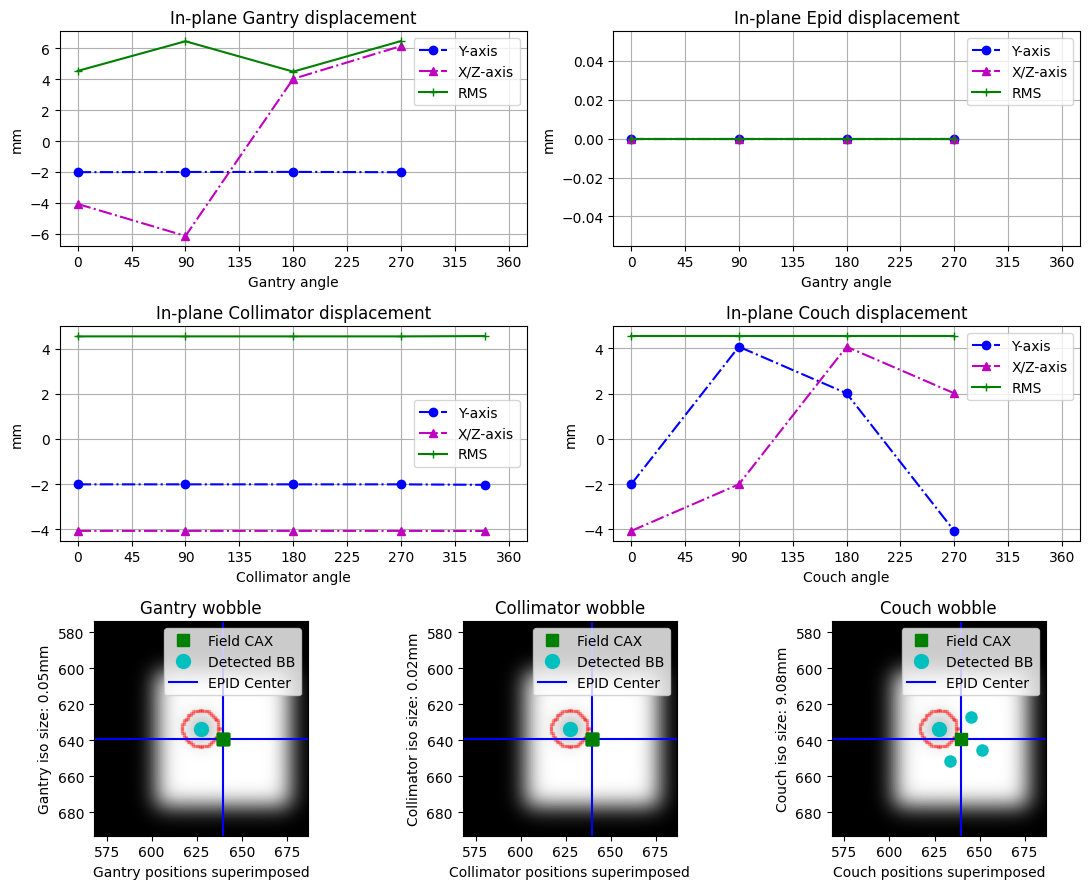
\includegraphics[width=0.85\textwidth]{Content/Images/analysis_wl_artificial_summary_plot.png}
    \caption{Summary plot of test with artificial images}
\end{figure}

\begin{figure}[H]
    \centering
    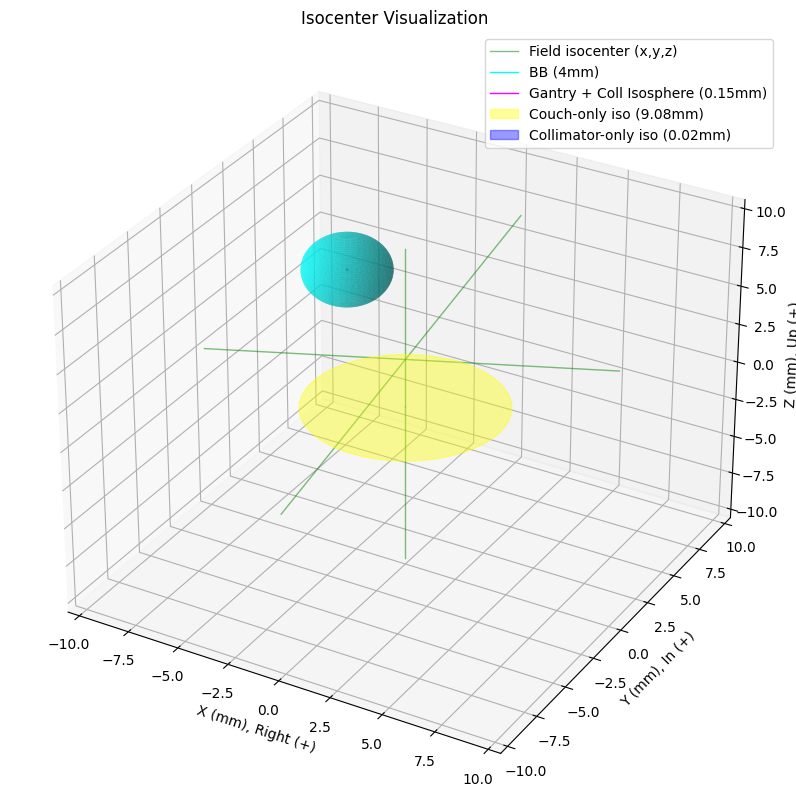
\includegraphics[width=0.60\textwidth]{Content/Images/analysis_wl_artificial_isocenter_plot.png}
    \caption{Isocenter plot of test with artificial images}
\end{figure}

\subsubsection{Analysis}

The results are highly in line with the predictions, showing a significant deviation of BB from the norm. As can be seen in the visualisation, with these parameters the device, the isocentres are not aligned, and thus it can be concluded, that the device is not correctly calibrated, as anticipated.

\section{Leaves analysis}

\subsection{Real image with correctly calibrated leaves} \label{sec:laExampleCalibrated}

This analysis is conducted on a real DICOM image obtained with the device from the National Institute of Oncology in Kraków (\autoref{sec:envSetupOncologyKrakow}).

\subsubsection{Numerical inputs}

\begin{itemize}

    \item Horizontal real size of an image (x): 428.8mm

    \item Vertical real size of an image (y): 428.8mm
    
    \item Tolerance x: 2 px

    \item Tolerance y: 2 px

    \item Permitted errors per leaf: 1

    \item Binarisation threshold: 215

    \item SE size: 25 px

    \item Sobel kernel size: 1 px
    
\end{itemize}

\subsubsection{Leaves definition}

Leaves have been defined to correspond to their intended arrangement (\autoref{fig:laPlanOncology}). The radiation field comprises a total of 60 leaves, of which 32 are 2.5 mm wide and 28 are 5 mm wide. The thinner leaves are concentrated in the centre of the field, allowing more precise modelling of the field. The thicker leaves are located at both ends of the field, with 14 at the top and 14 at the bottom. In the middle of the radiation field, the leaves form a square with a side of 10mm.

\begin{figure}[H]
    \centering
    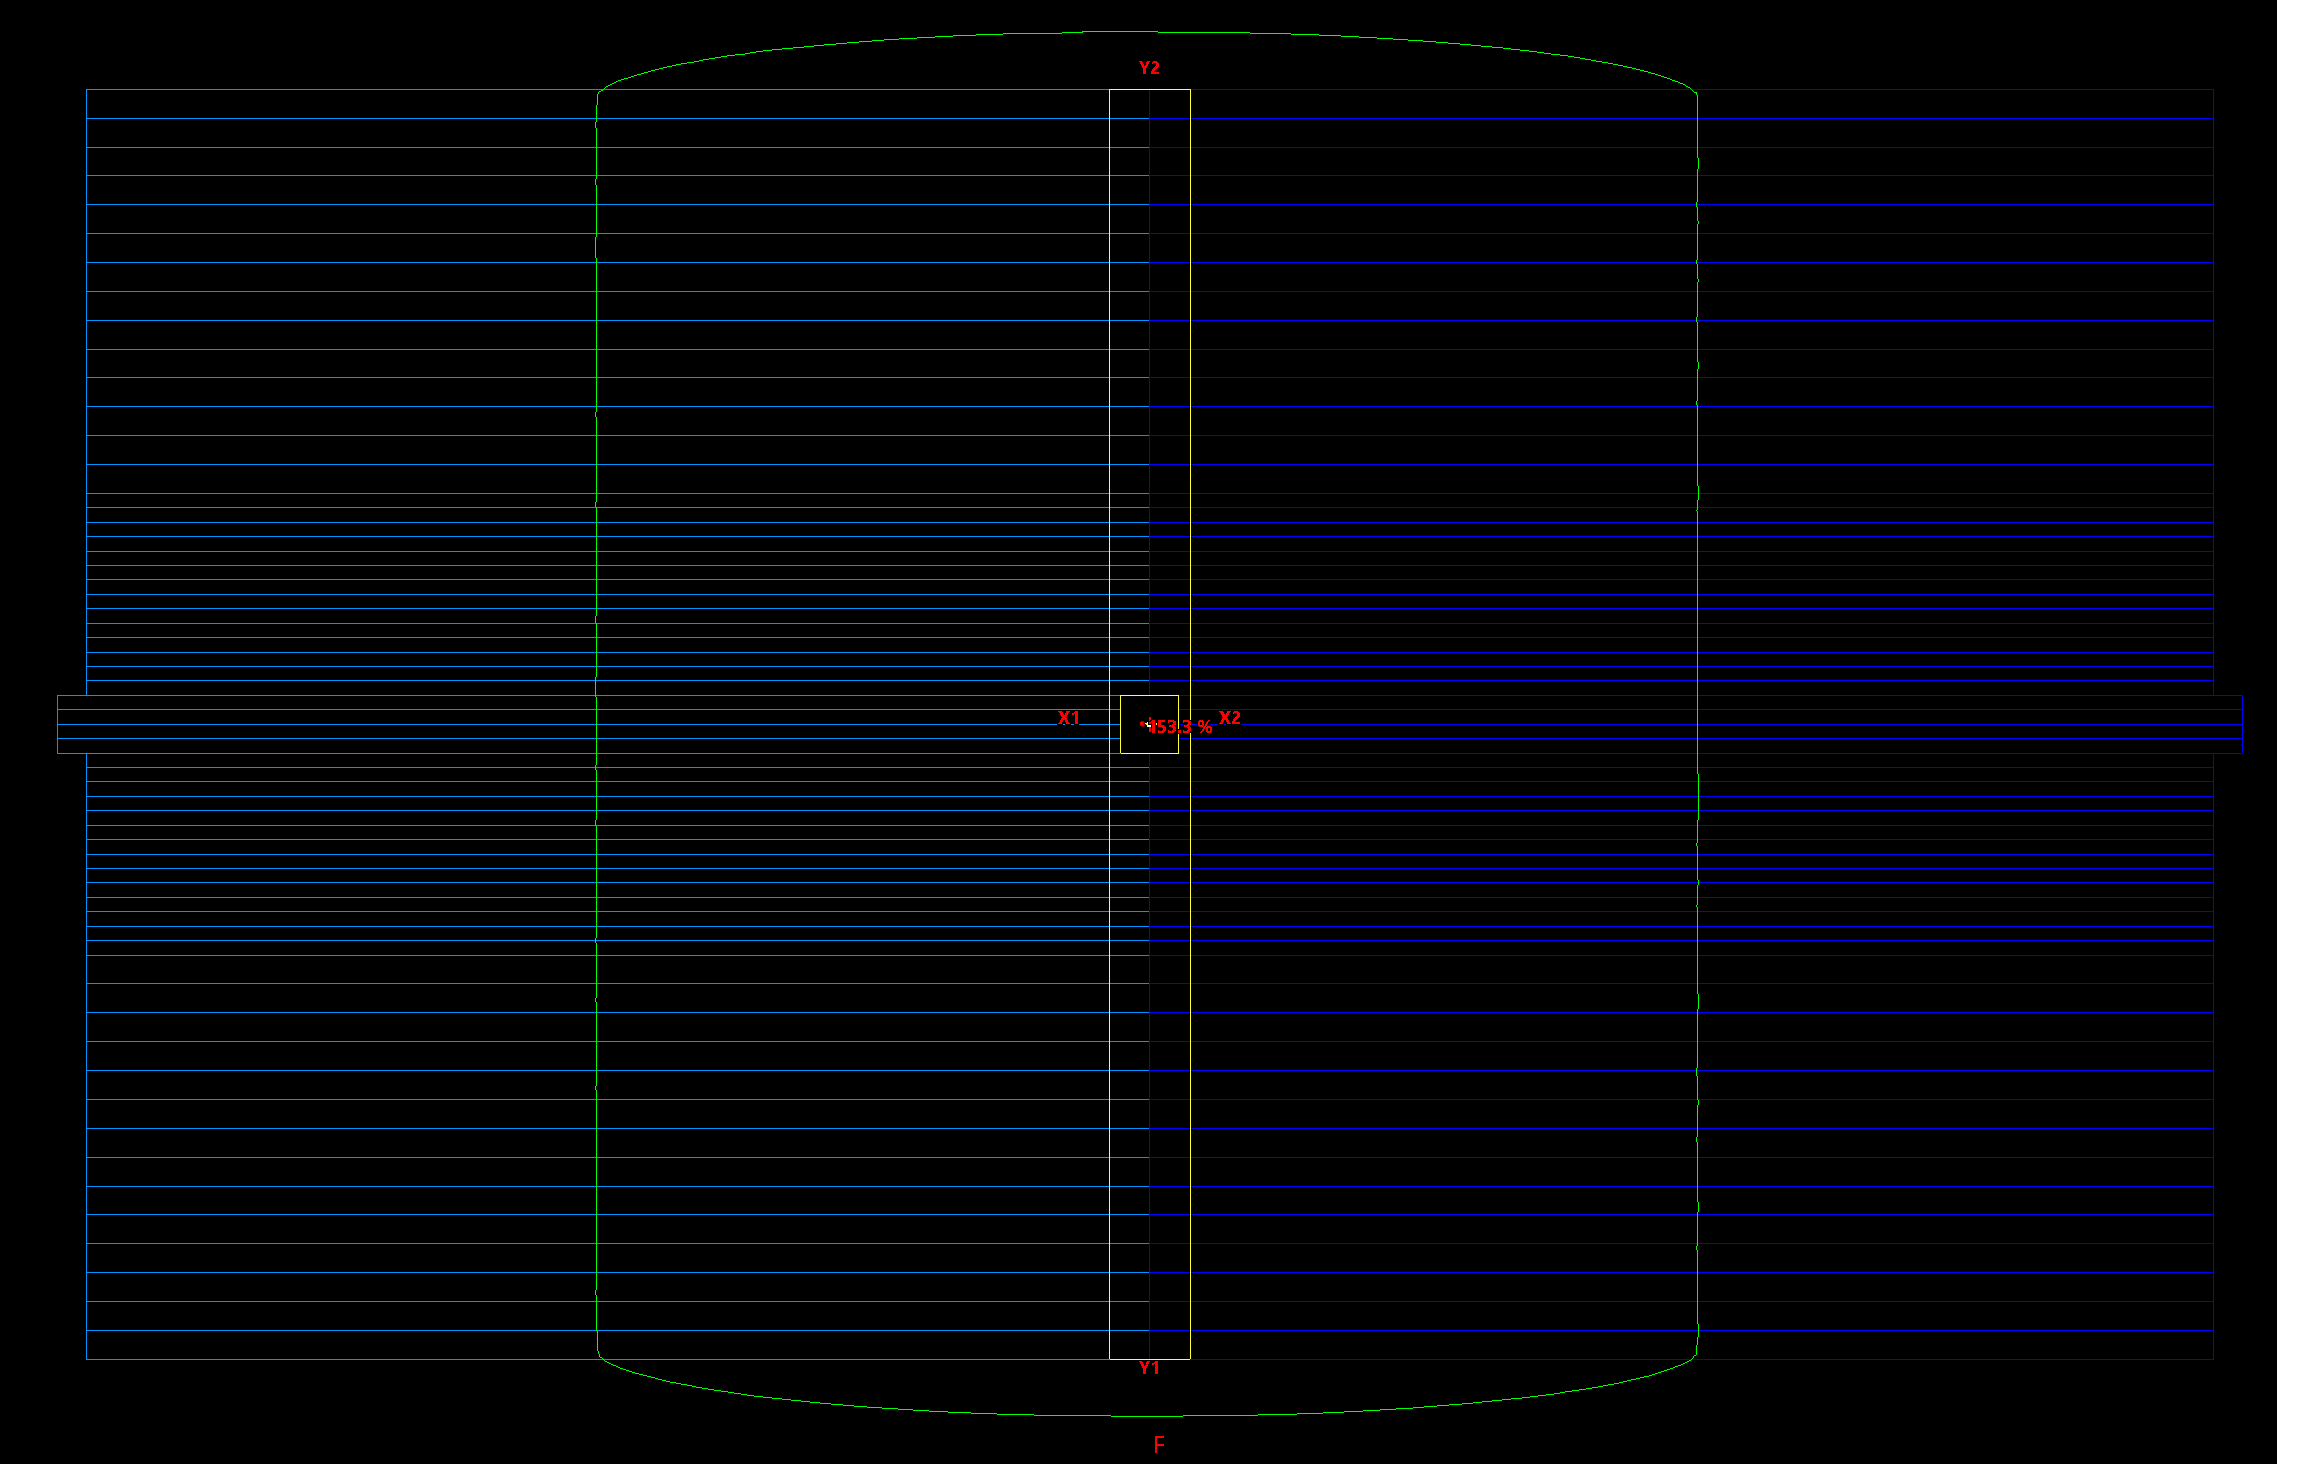
\includegraphics[width=1\textwidth]{Content/Images/analysis_la_plan.png}
    \caption{Leaves alignment from example plan}
    \label{fig:laPlanOncology}
\end{figure}

\subsubsection{Input image}

\begin{figure}[H]
    \centering
    \fbox{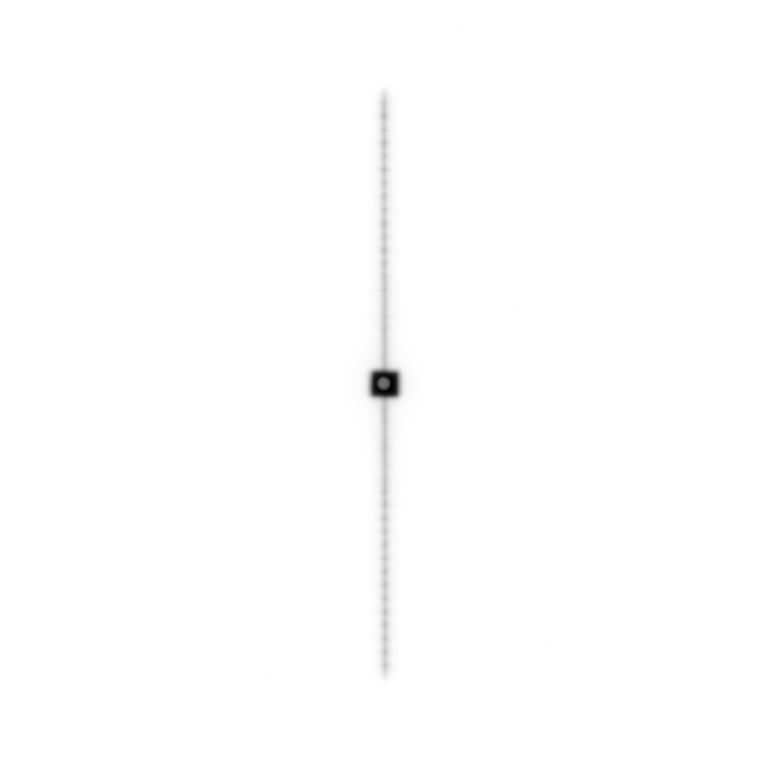
\includegraphics[width=0.6\textwidth]{Content/Images/analysis_la_oncology_input_image.png}}
    \caption{LA analysis input image}
\end{figure}

\subsubsection{Results}

\begin{figure}[H]
    \centering
    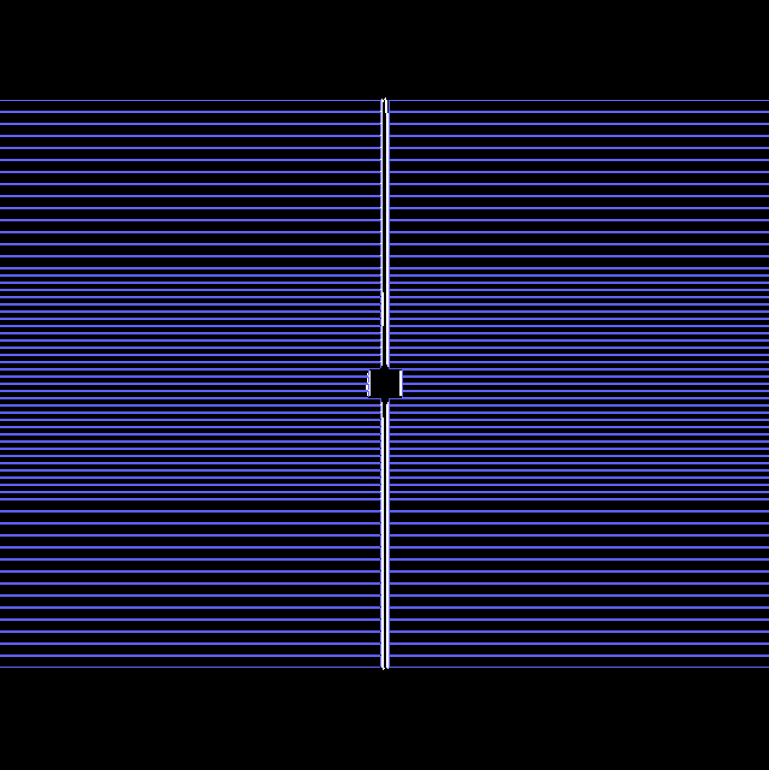
\includegraphics[width=0.65\textwidth]{Content/Images/analysis_la_oncology_preprocessed_image.png}
    \caption{Preprocessed image}
\end{figure}

\begin{figure}[H]
    \centering
    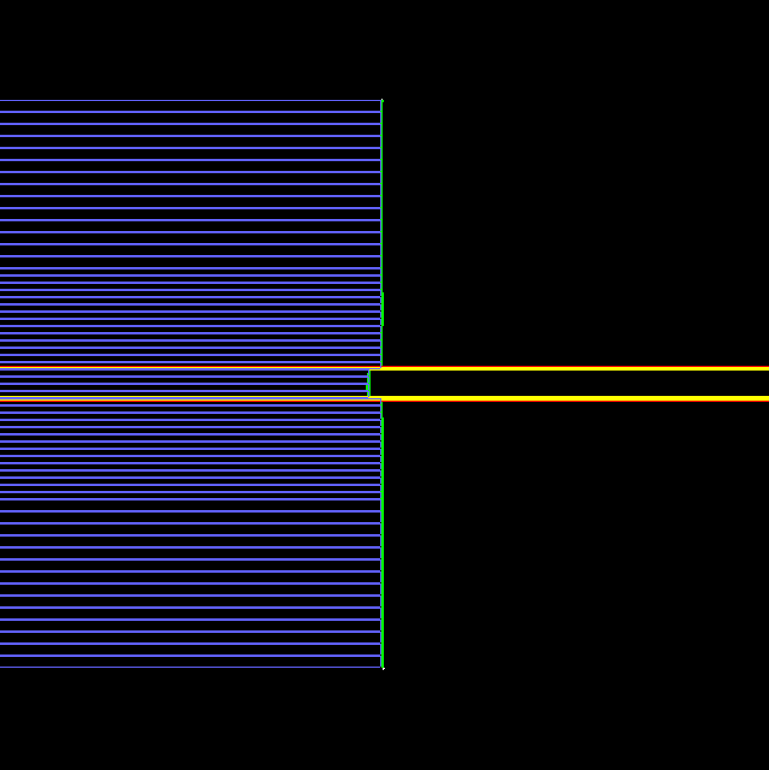
\includegraphics[width=0.65\textwidth]{Content/Images/analysis_la_oncology_left_leaves.png}
    \caption{Analyzed leaves left}
\end{figure}

\begin{figure}[H]
    \centering
    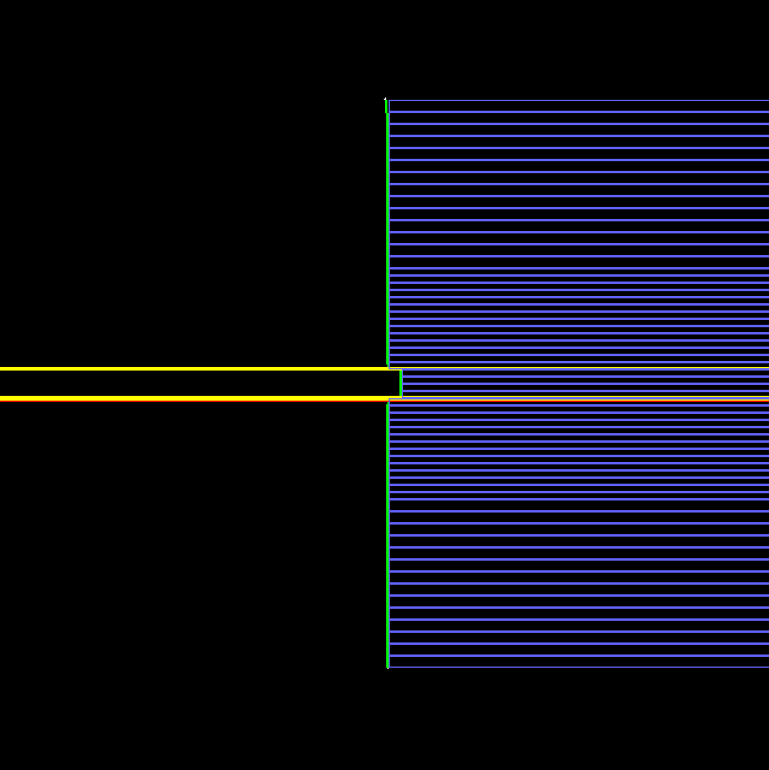
\includegraphics[width=0.65\textwidth]{Content/Images/analysis_la_oncology_right_leaves.png}
    \caption{Analyzed leaves right}
\end{figure}

\subsubsection{Detected faulty leaves}

The algorithm detected no faulty leaves.

\subsubsection{Analysis}

As can be seen, no faulty leaves were detected in this case. In the resulting images, two places can be seen, near the edges of the radiation field, where no edge was detected (yellow and red horizontal stripes). This is due to imperfections in the edge detection algorithm at the point of sharp changes in their direction. However, these imperfections are within the tolerances, that is, the number of counted errors (red) is less than the limit, and are therefore not considered as non-calibrated leaves. Erroneous values close to the edges of the leaves have been correctly marked in yellow and are not counted as errors. Consequently, based on the test, it can be concluded that the leaves are correctly calibrated.

\subsection{Real image with incorrectly calibrated leaves}

In this analysis, the input image is identical to that used in \autoref{sec:laExampleCalibrated}, but the definition of the leaves has been modified artificially to introduce faulty leaves to demonstrate how the algorithm will behave and what the results will look like in such a situation.

\subsubsection{Inputs definition}

The input image and numerical inputs are the same as in \autoref{sec:laExampleCalibrated}. The left side of the leaves definition is similar to that of \autoref{sec:laExampleCalibrated}, with the difference that the x position of the edge of the two leaves has been changed. One has been extended to the left by 50 pixels, while the other has been extended to the right by 10 pixels. The right side has been replaced by 3 big leaves which group together adjacent leaves, to visualise the problem better.

\subsubsection{Result images}

\begin{figure}[H]
    \centering
    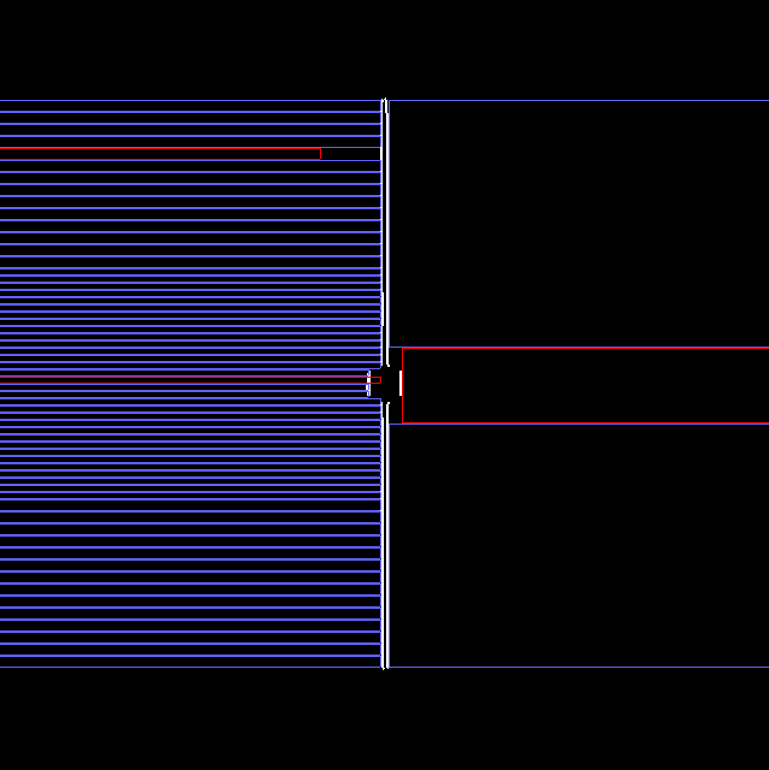
\includegraphics[width=0.65\textwidth]{Content/Images/analysis_la_faulty_preprocessed_image.png}
    \caption{Preprocessed image}
\end{figure}

\begin{figure}[H]
    \centering
    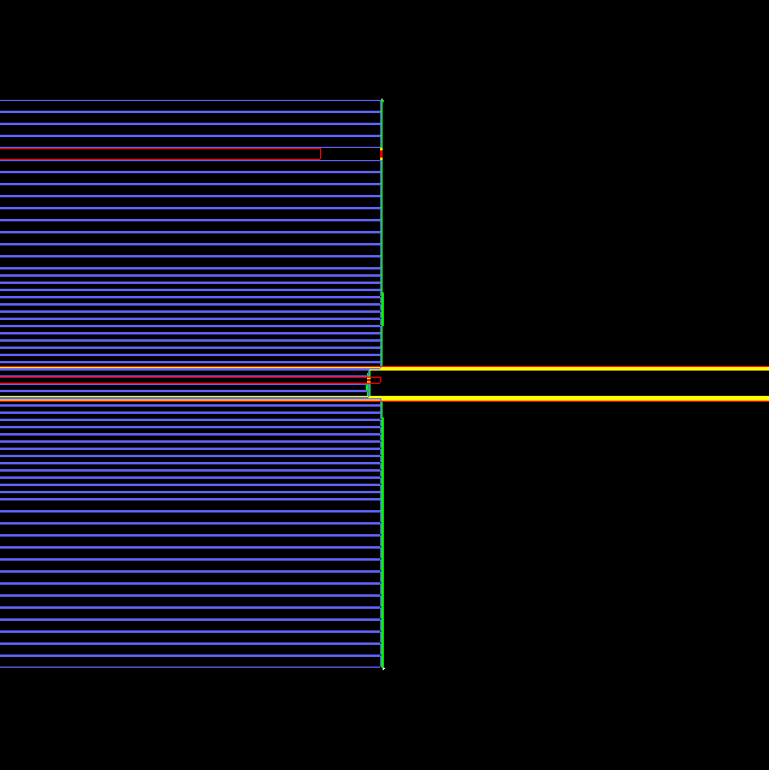
\includegraphics[width=0.65\textwidth]{Content/Images/analysis_la_faulty_left_leaves.png}
    \caption{Analyzed leaves left}
\end{figure}

\begin{figure}[H]
    \centering
    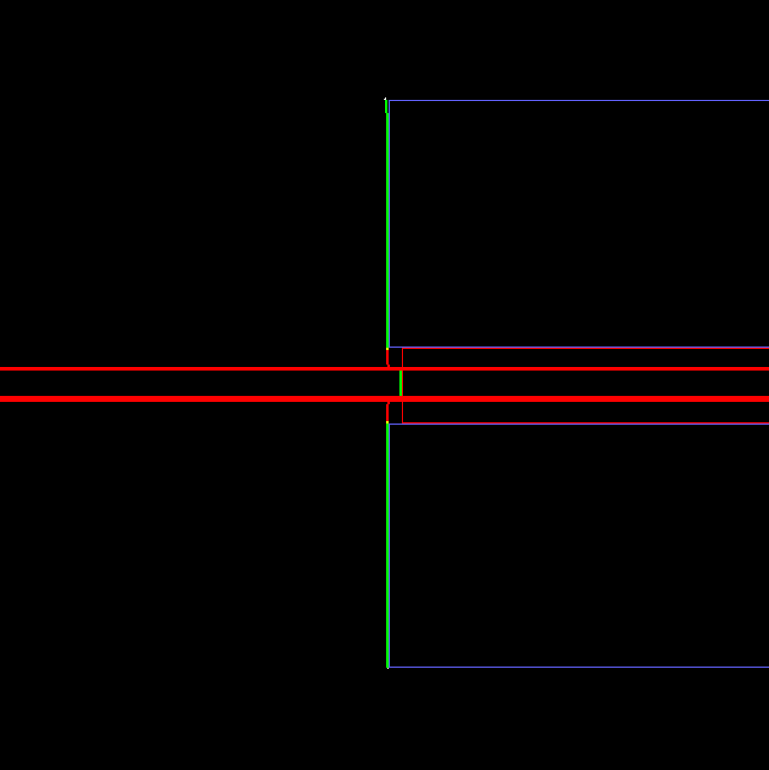
\includegraphics[width=0.65\textwidth]{Content/Images/analysis_la_faulty_right_leaves.png}
    \caption{Analyzed leaves right}
\end{figure}

\subsubsection{Faulty leaves}

The algorithm detected 3 faulty leaves, 2 on the left and 1 on the right. The top left faulty leaf has a mean deviation of 33.4mm (50px), the bottom left faulty leaf has a mean deviation of 6mm (9px), and the right faulty leaf has a mean deviation of 8mm (12px).

\subsubsection{Analysis}

As can be observed, the algorithm correctly identified all three miscalibrated leaves. Both left leaves were successfully detected, along with their respective deviations. For the upper leaf, the detected deviation is precisely the amount by which the leaf was shifted. For the lower leaf, there is a discrepancy of one pixel, from the set up and detected positions. This is expected, given that the detected leaf edge thickness exceeds one pixel, thereby reducing the detected distance.

As for the right side, the algorithm also correctly detected a slightly more difficult case, where the detected edges indicate that the leaf should be thinner than defined. Even though the centre of the leaf is at the correct offset, the number of erroneous values closer to the edge exceeds the allowed amount, with the result that the leaf is classified as faulty. It is worth noting that also in this case, the algorithm correctly maintains the tolerance of the nearest points near the edge of the leaf definition.
